\documentclass[titlepage, a4paper]{article}
%importerat (2017-01-24) layout-bibliotek från Hannes Snögren, KMM 14/15. Med godkännande från honom. 
%ändrat i settings sedan dess. babel-bibliotek för swedish krävs för kompilering.
%debian: sudo apt-get install texlive-lang-european

\usepackage[swedish]{babel}
\usepackage[utf8]{inputenc}
\usepackage{color}
\usepackage{graphicx}
\usepackage{etoolbox}
\usepackage{hyperref}
\usepackage{calc}  
\usepackage{enumitem}
\usepackage{titlesec}

\makeatletter
\patchcmd{\ttlh@hang}{\parindent\z@}{\parindent\z@\leavevmode}{}{}
\patchcmd{\ttlh@hang}{\noindent}{}{}{}
\makeatother

%Spacing för sections och subsections
\titlespacing*{\section}
{0pt}{5.5ex plus 1ex minus .2ex}{1.0ex plus .2ex}
%\titlespacing*{\subsection}
%{0pt}{5.5ex plus 1ex minus .2ex}{4.3ex plus .2ex}

% Sidformat
\usepackage{a4wide}

% Fixa Appendix-titlar
\usepackage[titletoc,title]{appendix}

% Bättre tabeller
\usepackage{tabularx}

% Bättre bildtexter
\usepackage[margin=10pt,font=small,labelfont=bf,labelsep=endash]{caption}

% Enkelt kommando som låter mig attgöra-markera text
\newcommand{\todo}[1] {\textbf{\textcolor{red}{#1}}}

% Nytt \paragraph låter oss ha onumrerade bitar
\makeatletter
\renewcommand\paragraph{\@startsection{paragraph}{4}{\z@}%
{-3.25ex\@plus -1ex \@minus -.2ex}%
{1.5ex \@plus .2ex}%
{\normalfont\normalsize\bfseries}}
\makeatother

\providecommand{\LAYOUTlogga}{../mall/Logga.png}
\providecommand{\LAYOUTdatum}{\today}


%% Headers och Footers
\usepackage{fancyhdr}
\pagestyle{fancy}
\lhead{\includegraphics[scale=0.12]{\LAYOUTlogga}}
\setlength{\headsep}{0.4in}
\rhead{\ifdef{\LAYOUTutfardare}{Utfärdat av \LAYOUTutfardare \\\LAYOUTdatum}\LAYOUTdatum}
\lfoot{\LAYOUTkursnamn \\ \LAYOUTdokumenttyp}
\cfoot{\thepage}
\rfoot{\LAYOUTprojektgrupp \\ \LAYOUTprojektnamn}

%% Titelsida
\newcommand{\LAYOUTtitelsida}{%
{\ }\vspace{45mm}
\begin{center}
  \textbf{\Huge \LAYOUTdokument}
\end{center}
\begin{center}
  {\Large Redaktör: \LAYOUTredaktor}
\end{center}
\begin{center}
  {\Large \textbf{Version \LAYOUTversion}}
\end{center}
\vspace{5mm}
\ifdef{\LAYOUTfrontpicture}{
\begin{center}
    \LAYOUTfrontpicture
\end{center}
}

\newpage
}


% Projektidentitet
\newenvironment{LAYOUTprojektidentitet}{%
{\ }\vspace{45mm}
\begin{center}
  {\Large PROJEKTIDENTITET}\\[0.5ex]
  {\small
  \LAYOUTartaltermin, \LAYOUTprojektgrupp\\
  Linköpings Tekniska Högskola, IDA
  }
\end{center}
\begin{center}
  {\normalsize Gruppdeltagare}\\
  \def\arraystretch{1.5}%
  \begin{tabular}{|l|l|p{25mm}|l|}
    \hline
    \textbf{Namn} & \textbf{Ansvar} & \textbf{Telefon} & \textbf{E-post} \\
    \hline
}%
{%
    \hline
  \end{tabular}
\end{center}
\begin{center}
  {\small
    \ifdef{\LAYOUTgruppadress}{\textbf{E-postlista för hela gruppen}: \LAYOUTgruppadress\\}{}
    \ifdef{\LAYOUTgrupphemsida}{\textbf{Hemsida}: \LAYOUTgrupphemsida\\[1ex]}{}
    \ifdef{\LAYOUTkund}{\textbf{Kund}: \LAYOUTkund\\}{}
    \ifdef{\LAYOUTkundkontakt}{\textbf{Kontaktperson hos kund}: \LAYOUTkundkontakt\\}{}
    \ifdef{\LAYOUTkursansvarig}{\textbf{Kursansvarig}: \LAYOUTkursansvarig\\}{}
    \ifdef{\LAYOUThandledare}{\textbf{Handledare}: \LAYOUThandledare\\}{}
  }
\end{center}
\newpage
}
\newcommand{\LAYOUTgruppmedlem}[4]{\hline {#1} & {#2} & {#3} & {#4} \\}

%% Dokumenthistorik
\newenvironment{LAYOUTdokumenthistorik}{%
\begin{center}
  Dokumenthistorik\\[1ex]
  %\begin{small}
  \def\arraystretch{1.5}%
    \begin{tabular}{|l|l|p{45mm}|p{30mm}|l|}
      \hline
      \textbf{Version} & \textbf{Datum} & \textbf{Utförda förändringar} & \textbf{Utförda av} & \textbf{Granskad} \\
      }%
    {%
			\hline
    \end{tabular}
  %\end{small}
\end{center}
}

\newcommand{\LAYOUTversionsinfo}[5]{\hline {#1} & {#2} & {#3} & {#4} & {#5} \\}

% Kravlistor
\newenvironment{LAYOUTkravlista}{
	\center
		\tabularx{\textwidth}{| p{1.2cm} | p{1.9cm} | X | c |}
			\hline
			\textbf{Krav} & \textbf{Förändring} & \textbf{Beskrivning} & \textbf{Prioritet} \\\hline
}
{
		\endtabularx
	\endcenter
}

\newcounter{LAYOUTkravnummer}
\addtocounter{LAYOUTkravnummer}{1}
\newcommand{\LAYOUTkrav}[4][Krav \arabic{LAYOUTkravnummer}]{{#1} & {#2} & {#3} & {#4} \stepcounter{LAYOUTkravnummer}\\\hline}

% Milstolps-lista
\newenvironment{LAYOUTmilstolpar}{
	\center
		\tabularx{\textwidth}{| p{1.2cm} | X | l |}
			\hline
			\textbf{Nr} & \textbf{Beskrivning} & \textbf{Datum} \\\hline
}
{
		\endtabularx
	\endcenter
}

\newcounter{LAYOUTstolpnummer}
\addtocounter{LAYOUTstolpnummer}{1}
%\newcommand{\LAYOUTmilstolpe}[3][Krav \arabic{LAYOUTstolpnummer}]{{#1} & {#2} & {#3} \stepcounter{LAYOUTstolpnummer}\\\hline}
\newcommand{\LAYOUTmilstolpe}[3]{{#1} & {#2} & {#3} \\\hline}

% Aktivitets-lista
\newenvironment{LAYOUTaktivitetslista}{
	\center
		\tabularx{\textwidth}{| p{0.3cm} | X | c | c |}
			\hline
			\textbf{Nr} & \textbf{Beskrivning} & \textbf{Beroende av} & \textbf{Timmar} \\\hline
}
{
		\endtabularx
	\endcenter
}

\newcounter{LAYOUTaktivitetsnummer}
\addtocounter{LAYOUTaktivitetsnummer}{1}
% \newcommand{\LAYOUTaktivitet}[4][\arabic{LAYOUTstolpnummer}]{{#1} & {#2} & {#3} & {#4} \stepcounter{LAYOUTstolpnummer}\\\hline}
\newcommand{\LAYOUTaktivitet}[4]{{#1} & {#2} & {#3} & {#4} \\\hline}

% Mall för mötesprotokoll
\newenvironment{projektmote}[2]{
  {\ }\vspace{5mm}

  \centerline{\textbf{\Huge #1}}
  \vspace{2mm}
  \centerline{\LARGE #2}
  \vspace{10mm}

  \begin{itemize}
}
{
  \end{itemize}
}

\newcounter{paragrafnummer}
\addtocounter{paragrafnummer}{1}
\newcommand{\paragraf}[1]{\item{\textsection \arabic{paragrafnummer}. {#1}}\addtocounter{paragrafnummer}{1}}

% Mall för Statusrapport
\newenvironment{statusrapport}{
  \center
    \tabularx{\textwidth}{| p{0.4cm} | X | X | p{14.5mm} | p{13.5mm} | p{16.5mm} | p{16.5mm} |}
    \hline
    \textbf{Nr} & \textbf{Aktivitet} & \textbf{Beroenden} & \textbf{Planerad tid} & \textbf{Nedlagd tid} & \textbf{Planerad klar} & \textbf{Beräknat klart} \\\hline
}
{
    \endtabularx
  \endcenter
}

\newcommand{\aktivitetstatus}[7]{{#1} & {#2} & {#3} & {#4} & {#5} & {#6} & {#7} \\\hline}


%parametrar som behövs för layout
\newcommand{\LAYOUTredaktor}{Rebecca Lindblom}
\newcommand{\LAYOUTversion}{1.5}
\newcommand{\LAYOUTdokument}{Kravspecifikation}
\newcommand{\LAYOUTdokumenttyp}{Kravspecifikation}
\newcommand{\LAYOUTgranskatdatum}{}
\newcommand{\LAYOUTgranskare}{}
\newcommand{\LAYOUTgodkannare}{}
\newcommand{\LAYOUTgodkantdatum}{}
\newcommand{\LAYOUTkursnamn}{TDDD96}
\newcommand{\LAYOUTprojektnamn}{Visualization}
\newcommand{\LAYOUTprojektgrupp}{Grupp 2}
\newcommand{\LAYOUTartaltermin}{VT 2017}
\newcommand{\LAYOUTgrupphemsida}{https://gitlab.ida.liu.se/tddd96/visualization}
\newcommand{\LAYOUTkund}{Kristian Sandahl, Ola Leifler}
\newcommand{\LAYOUTkundkontakt}{Kristian Sandahl}
\newcommand{\LAYOUTkursansvarig}{Kristian Sandahl}
\newcommand{\LAYOUThandledare}{Lena Buffoni}

%override paket för detta doc.
\usepackage[swedish]{babel}
\usepackage{pdfpages}
\usepackage{tikz}
\usepackage{adjustbox}
\usetikzlibrary{shapes, arrows}
\usepackage{graphicx}
\graphicspath{ {../../images/} }
\pagenumbering{roman}
\DeclareGraphicsRule{.0.pdf}{pdf}{*}{}
\usepackage{biblatex}
\usepackage{ulem}
\addbibresource{../mall/references.bib}

\begin{document}

\LAYOUTtitelsida

\begin{LAYOUTprojektidentitet}
\LAYOUTgruppmedlem{Johan Nåtoft}{Teamledare}{070-7661443}{johna702@student.liu.se}
\LAYOUTgruppmedlem{Joakim Argillander}{Testledare}{076-8618641}{joaar286@student.liu.se}
\LAYOUTgruppmedlem{Victor Bodin}{Kvalitetssamordnare}{073-5183199}{vicbo282@student.liu.se}
\LAYOUTgruppmedlem{Sebastian Callh}{Utvecklingsledare}{073-8204664}{sebca553@student.liu.se}
\LAYOUTgruppmedlem{Rebecca Lindblom}{Analysansvarig}{073-4364079}{rebli156@student.liu.se}
\LAYOUTgruppmedlem{Johan Thornström}{Arkitekt}{070-5297445}{johth918@student.liu.se}
\LAYOUTgruppmedlem{Jonathan Wahlund}{Konfigurationsansvarig}{070-6106911}{johwa732@student.liu.se}
\LAYOUTgruppmedlem{Daniel Wassing}{Dokumentansvarig}{076-7741110}{danwa223@student.liu.se}
\end{LAYOUTprojektidentitet}



\begin{LAYOUTdokumenthistorik}
\LAYOUTversionsinfo{0.1}{2017-01-25}{Upprättande av dokument}{Daniel Wassing}{}
\LAYOUTversionsinfo{0.2}{2017-02-01}{Första utkast inför tekniskt möte}{Kravspecgruppen}{Lena}
\LAYOUTversionsinfo{0.3}{2017-02-09}{Upprättande av majoritet av krav efter tekniskt möte.}{Rebecca, Sebastian, Joakim}{Rebecca}
\LAYOUTversionsinfo{1.0}{2017-02-20}{Uppdatering av krav efter handledar- och kundmöte samt intervju.}{Rebecca, Sebastian, Joakim}{Rebecca}
\LAYOUTversionsinfo{1.1}{2017-03-06}{Uppdatering efter kundmöte och visning av första prototyp, samt uppdatering av kravförändringar}{Rebecca}{Sebastian}
\LAYOUTversionsinfo{1.2}{2017-03-09}{Tillägg i definition av händelseförlopp, omformuleringar av funktionella krav efter visning av andra prototyp.}{Rebecca}{Daniel}
\LAYOUTversionsinfo{1.3}{2017-03-27}{Tillägg av funktionella krav enligt prototyp presenterad för kund. Rubrik i avsnitt 3 omformulerad från \textit{Specifika krav} till \textit{Krav}. Ändrad prioritet på tre st krav.}{Sebastian}{Rebecca}
\LAYOUTversionsinfo{1.4}{2017-04-29}{Förändring av krav för placering av muspekare över nod, förändring och tillägg av krav för tidsvisualisering.}{Rebecca}{Victor}
\LAYOUTversionsinfo{1.5}{2017-05-15}{Krav på intervallsbredd i tidslinjen borttaget, samt möjlighet för användaren att se genomsnittlig grad av testfallsresultat i testsviter. Ny logotype inlagd.}{Rebecca}{Victor}
\end{LAYOUTdokumenthistorik}

\newpage
\tableofcontents	%Innehållsförteckning

\newpage
\pagenumbering{arabic} %Påbörja sidnumrering

%https://www.ida.liu.se/~TDDC88/theory/03requirements.pdf
% Counter för kravnumrering:
% Innan varje krav läggs en \addtocounter{req_num}{1}.
% Denna måste ligga precis efter \hline i tabellen och INTE efter cellens innehåll (--> compile error).
\newcounter{req_num}
\setcounter{req_num}{0}

%inputs go here
% Ordlista ska ej med i innehållsförteckningen
\section*{Ordlista}
Här följer förklaring av förkortningar som används genom hela detta dokument.
\begin{description}[leftmargin=!,labelwidth=\widthof{\bfseries Some text}]
\item[CI] Continous Integration
\item[IDA] Institutionen för Datateknik vid Linköpings Universitet
\end{description}
\newpage
\section{Introduktion}
Följande dokument utgör en kravspecifikation för projektet. 
\subsection{Syfte och målgrupp}
Syftet med kravspecifikationen är att tydliggöra alla projektets intressenters krav på applikationen. Kravspecifikationen utgör ett konstruktionsunderlag såväl som underlag för dokumentation och testning av applikationen. Kravspecifikationen ska användas som beslutsunderlag för när beslut ska tas om projektet.
\\
\\
Målgruppen för dokumentet är alla projektets intressenter, däribland beställare, utvecklare och testare. 
\subsection{Avgränsningar}
Applikationen är ett verktyg för visualisering och utför således ingen databehandling. Den behöver heller inte fungera på mindre skärmar och handhållna enheter eller stödja andra språk än engelska.

\begin{table}[h!]
  \centering
  \caption{En tabell över utvecklingsplattformar.}
  \def\arraystretch{1.5}
  \begin{adjustbox}{max width=\textwidth}
    \begin{tabularx}{\textwidth}{ | l | X | }
      \hline
      \textbf{Operativsystem} & \textbf{Webbläsare} \\
      \hline
      Ubuntu 16.04 & Firefox 51.0.1 \\
      \hline
      macOS Sierra 10.12.3 & Chrome 55.0.2883.95 \\
      \hline
      Windows 8.1, 10 & Chrome 55.0.2883.95 \\
      \hline
    \end{tabularx}
  \end{adjustbox}
  \label{tab:utvecklingsplattformar}
\end{table}
\ \\
Utvecklingen och testning kommer ske på de plattformar som ses i tabell \ref{tab:utvecklingsplattformar} och applikationen är därmed inte garanterad att fungera på andra plattformar. Applikationen kommer att utvecklas som en forskningsprototyp.

\subsection{Dokumentkonventioner}
\subsubsection{Format på krav}
Kraven på produkten kommer att anges löpande i de olika avsnitten.

\begin{table}[h!]
  \centering
  \caption{En tabell över format på krav.}
  \def\arraystretch{1.5}
  \begin{adjustbox}{max width=\textwidth}
    \begin{tabularx}{\textwidth}{ | c | l | X | c | }
      \hline
      Kravnummer & Förändring & Kravtext & Prioritet \\
      \hline
    \end{tabularx}
  \end{adjustbox}
  \label{tab:krav_format}
\end{table}
\ \\
Kraven på produkten ges på följande form enligt tabell \ref{tab:krav_format}. Alla krav numreras från K1 och framåt där K indikerar att det är ett krav. Förändring indikerar om kravet är annorlunda från originalkravet. Kravtext ger information om kravet. Prioritet anger om kravet är ett baskrav som uppfylls under utvecklingsiteration 1 (prioritet 1), eller ett krav som uppfylls i en senare utvecklingsinteration (prioritet 2), eller om det är ett krav vid eventuell vidareutveckling (prioritet 3).

\newpage
\subsubsection{Definitioner}
Här följer förklaring av ord som används genom hela detta dokument.

\begin{description}[leftmargin=!,labelwidth=\widthof{\bfseries Continous Integration}]
\item[Artefakt] En faktiskt produkt, t.ex. en JavaScript-klass eller ett dokument.
\item[Commit] En uppsättning ändringar i ett versionshanteringssystem.
\item[Continous Integration] Arbetsmetodik för att kontinuerligt integrera, bygga och testa systemändringar.
\item[Chrome] Webbläsare.
\item[Eiffel] Ramverk från Ericsson som i det här projektet används för att spåra händelser i CI-system. Ramverket har länge används internt på Ericsson men blev nyligen publikt. Eiffel som helhet har inga versioner, det system som används i projektet är det som finns publicerat i commit 0303cf3. \cite{website:eiffel}
\item[Firefox] Webbläsare.
\item[Händelseförlopp] Beskriver den kedja av händelser som sker p.g.a. en ändring i ett CI-system. Kedjan initeras av en kodändring och begränsas av att en pålitlighetsgrad sätts.
\item[JavaScript] Programmeringsspråk som i projektet används för att skriva applikationen.
\item[macOS] Operativsystem.
\item[Meteor] Ramverk för webbutveckling som använder JavaScript. Version 1.4.2.6 används i detta projekt. \cite{website:meteor}
\item[Pålitlighetsgrad] Mått på hur väl en artefakt presterat vid testning.
\item[README-fil] Fil med information om en applikation, t.ex. hur den används eller systemkrav.
\item[Repository, repo] Lagringsutrymme för versionshanterade artefakter.
\item[Ubuntu] Operativsystem.
\item[Windows] Operativsystem.
\end{description}

\subsection{Översikt}
Kravspecifikationen innehåller en beskrivning av produkten där en tolkning av kundkraven har gjorts och dess funktioner och användaregenskaper beskrivs. Kravspecifikationen innehåller också de specifika krav som formulerats utifrån den tolkning som gjorts av kundens krav och önskemål beträffande gränssnitt, funktioner och prestandakrav samt begränsningar.
\newpage
\section{Beskrivning}
Detta avsnitt ger en övergripande beskrivning av applikationen i sig, dess funktionalitet, dess tilltänkta användare samt begränsningar för applikationens utformning.

\subsection{Beskrivning av applikationen}
Applikationen är ett verktyg för att tydligt få en överblick över händelser och flöden i CI-processer för ett system, exempelvis byggen och tester. Applikationens målgrupp är företag som bedriver mjukvaruutveckling med större utvecklingsteam. Ett företag i målgruppen använder sig i dagsläget av CI och vill kunna upptäcka flaskhalsar och förbättra sitt arbetsflöde. Applikationen är en webbaserad tjänst skriven i JavaScript. Data som visualiseras i applikationen kan komma från valfritt CI-system via ramverket Eiffel. Händelser och flöden visualiseras genom interaktiva grafer där användaren kan välja att visa data i flera olika nivåer för att kunna dra slutsatser sitt utvecklingsflöde. 

\begin{figure}[h]
    \centering
    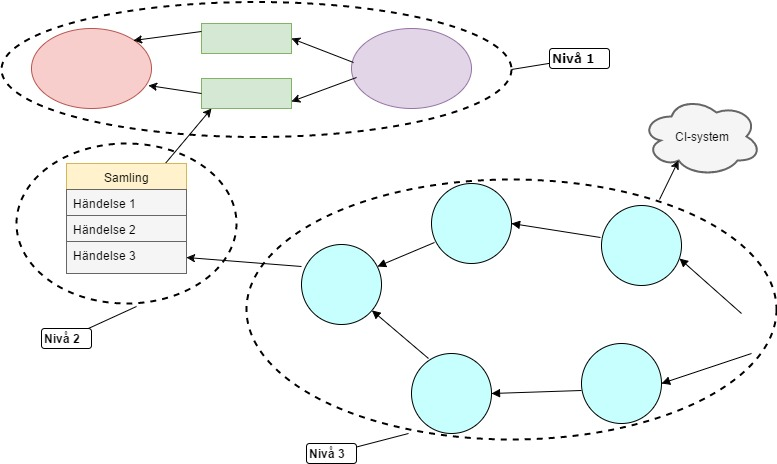
\includegraphics[width=\textwidth]{Visualization}
    \caption{De olika nivåerna av systemet, godtyckligt färgade.}
    \label{fig:system_overview}
\end{figure}
	
\subsection{Funktioner}
Applikationen har en aggregerad och sammanfattad vy av systemet (nivå 1 i figur \ref{fig:system_overview}). Varje nod i grafen på denna nivå representerar varsin typ av händelse, till exempel tester, byggen eller inspektioner. I denna vy slås alla händelser av samma typ samman till en nod. Användaren kan se en detaljerad samling av en viss typ av händelser genom att välja en nod i den aggregerade vyn (nivå 2 i figur \ref{fig:system_overview}). Genom att välja en av händelserna i samlingen kan användaren se ett händelseförlopp för den valda händelsen (nivå 3 i figur \ref{fig:system_overview}). I händelseförloppet kommer händelser som påverkat varandra att vara sammankopplade. 

\newpage

\subsection{Användaregenskaper}
Applikationen riktar sig till användare på alla nivåer inom mjukvaruutveckling, men främst till personer högre upp i hierarkin. Exempel på detta är projektledningen som får en översikt över mjukvaruutvecklingen.
\\ \\
Användaren bör ha god vana vid datorer i allmänhet, kunna navigera i och hantera en webbläsare samt ladda upp och ner filer till och från en hemsida. Användaren bör också vara välbekant med programvaruutveckling, begrepp inom CI, samt den programvara som systemet får sin data från. Användaren ska kunna läsa en README-fil med instruktioner för att installera en programvara. 

\subsection{Begränsningar}
Applikationen kommer köras i en webbläsare, därmed kommer prestandan begränsas av vad webbläsaren klarar av. Internetåtkomst kommer också krävas för att kunna använda applikationen. Renderingen kommer ske med hjälp av JavaScript vilket också kommer sätta ett tak för prestandan.

\subsection{Antaganden och beroenden}
Applikationen förlitar sig på att få Eiffel-data levererad till sig för att kunna utföra visualiseringen och hämtar alltså inte själv in någon data. Den kommer även att implementeras i JavaScript-ramverket Meteor vilket kräver att applikationens användare kan köra en modern JavaScript-applikation i sin webbläsare. Övriga beroenden kan komma att uppstå under projektets gång.
\newpage
\section{Krav}
Kravställningen på applikationen är ej absolut och kommer att utvärderas och ändras i överens-kommelse med kund. 

\subsection{Gränssnitt}
Eftersom applikationens enda uppgift är att presentera data så har den få gränssnitt.

\subsubsection{Användargränssnitt}
Applikationen byggs för att köras i en webbläsare på en persondator vilket är dess enda gränssnitt mot användaren.
\begin{table}[h!]
  \centering
  \caption{En tabell över applikationens krav på användargränssnitt.}
  \def\arraystretch{1.5}
  \begin{adjustbox}{max width=\textwidth}
    \begin{tabularx}{\textwidth}{ | c | l | X | c | }
      \hline
      \addtocounter{req_num}{1}
      K\arabic{req_num} & Orginal & Användaren ska kunna nå allt innehåll i applikationen med hjäp av mus och tangentbord. & 1 \\
      \hline
      \addtocounter{req_num}{1}
      K\arabic{req_num} & Ny i v. 1.0 & Gränssnittet ska vara användarvänligt, enligt testfall T01 i dokumentet Testplan. & 1 \\
      \hline
    \end{tabularx}
  \end{adjustbox}
  \label{tab:krav_interface}
\end{table}

\subsection{Funktionella krav}
\begin{table}[h!]
  \centering
  \caption{En tabell över applikationens funktionella krav.}
  \def\arraystretch{1.5}
  \begin{adjustbox}{max width=\textwidth}
    \begin{tabularx}{\textwidth}{ | c | l | X | c | }
      \hline
      \addtocounter{req_num}{1}
      K\arabic{req_num} & Hänv. till figur i v.1.1 & Applikationen ska kunna visa en graf med noder som representerar aggregerade händelser, motsvarande nivå 1 i figur \ref{fig:system_overview}. & 1 \\
      \hline
      \addtocounter{req_num}{1}
      K\arabic{req_num} & \parbox[t]{3.4cm}{Ny i v. 1.0\\Omformulerad i v. 1.2 och v. 1.5} & I den aggregerade grafen enligt K3 ska användaren kunna visa alla händelser i ett valt tidsintervall. & 1 \\
	  \hline
      \addtocounter{req_num}{1}
      K\arabic{req_num} & \parbox[t]{3.4cm}{Ny i v. 1.0\\Ändrad prio i v. 1.3} & Användaren ska kunna se om det existerar händelser utanför det valda tidsintervallet. & 2 \\     
      \hline
      \addtocounter{req_num}{1}
      K\arabic{req_num} & Ny i v. 1.0 & För händelser som har en status ska statusen visualiseras i färg. & 1 \\ 
      \hline
      \addtocounter{req_num}{1}
      K\arabic{req_num} & \parbox[t]{3.4cm}{Ny i v. 1.0\\Borttagen i v. 1.1} & \sout{Användaren ska kunna se händelsetyp och färgsättning för varje nod i en graf utan att behöva förflytta vyn.} & 1 \\
      \hline
      \addtocounter{req_num}{1}
      K\arabic{req_num} & \parbox[t]{3.5cm}{Ny i v. 1.0\\Omformulerad i v. 1.1\\Ändrad prio i v. 1.3} & Användaren ska kunna se händelsetyp och status i varje nod i den aggregerade grafen utan att behöva förflytta vyn. & 2 \\
      \hline
      \addtocounter{req_num}{1}
      K\arabic{req_num} & Omformulerad i v. 1.0 & Användaren ska kunna se pålitlighetsgrad för artefakter i aggregerade händelseförlopp. & 1 \\
      \hline
      \addtocounter{req_num}{1}
      K\arabic{req_num} & \parbox[t]{3.4cm}{Omformulerad i v. 1.0\\Ändrad prio i v. 1.3} & Användaren ska kunna se pålitlighetsgrad för artefakter i för ett händelseförlopp. & 2 \\
      \hline
    \end{tabularx}
  \end{adjustbox}
  \label{tab:krav_funk1}
\end{table}
\newpage

\begin{table}[h!]
  \centering
  \def\arraystretch{1.5}
  \begin{adjustbox}{max width=\textwidth}
    \begin{tabularx}{\textwidth}{ | c | l | X | c | }
    \hline
      \addtocounter{req_num}{1}
      K\arabic{req_num} & \parbox[t]{3.4cm}{Omformulerad i v. 1.1\\Omformulerad i v. 1.5} & Användaren ska kunna se grad av klarade och misslyckade testsviter i aggregerade händelseförlopp. & 1 \\
      \hline
      \addtocounter{req_num}{1}
      K\arabic{req_num} & Ny i v 1.1 & Användaren ska kunna se grad av klarade och misslyckade testfall för testsviter i ett händelseförlopp. & 1 \\
    \hline
      \addtocounter{req_num}{1}
      K\arabic{req_num} & Original & Användaren ska kunna se om testfall lyckats eller misslyckats i ett händelseförlopp. & 1 \\
      \hline
      \addtocounter{req_num}{1}
      K\arabic{req_num} & Hänv. till figur i v.1.1 & Användaren ska kunna välja en nod i den aggregerade grafen och presenteras med en detaljerad samling av händelser som noden representerar, motsvarande nivå 2 i figur \ref{fig:system_overview}. & 2 \\
      \hline
      \addtocounter{req_num}{1}
      K\arabic{req_num} & \parbox[t]{3.4cm}{Ny i v. 1.1\\Omformulerad i v. 1.2} & Användaren ska kunna välja en nod i den aggregerade grafen och bli presenterad med förändringar över tid hos nodens attribut, motsvarande nivå 2 i figur \ref{fig:system_overview}. & 2 \\
      \hline
      \addtocounter{req_num}{1}
      K\arabic{req_num} & Hänv. till figur i v.1.1 & Användaren ska kunna välja händelser i den detaljerade samlingen och presenteras med en graf som representerar dess händelseförlopp, motsvarande nivå 3 i figur \ref{fig:system_overview}. & 2 \\
      \hline
      \addtocounter{req_num}{1}
      K\arabic{req_num} & Original & Om användaren navigerar till ett händelseförlopp via en aggregerad graf ska hen kunna navigera tillbaka den aggregerade grafen. & 2 \\
      \hline
      \addtocounter{req_num}{1}
      K\arabic{req_num} & Original & Användaren ska kunna välja noder i händelseförloppet och länkas till programmet som genererade händelsen. & 2 \\
      \hline
      \addtocounter{req_num}{1}
      K\arabic{req_num} & Omformulerad i v. 1.4 & Användaren ska kunna utläsa utförandetid för händelser i ett händelseförlopp där data om utförandetid finns. & 2 \\
      \hline
      \addtocounter{req_num}{1}
      K\arabic{req_num} & Borttaget i 1.1 & \sout{Användaren ska kunna utläsa genomsnittlig tid mellan sammankopplade händelsetyper i den aggregerade vyn.} & 2 \\
      \hline
      \addtocounter{req_num}{1}
      K\arabic{req_num} & Ny i v. 1.0 & Om internetuppkopplingen försvinner under en användarsession ska användaren få en notis om det. & 2 \\
      \hline
      \addtocounter{req_num}{1}
      K\arabic{req_num} & Ny i v. 1.3 & Användaren ska kunna zooma in och ut i en graf med hjälp av ett grafiskt skjutreglage och genom att scrolla med musen. & 1 \\
      \hline
      \addtocounter{req_num}{1}
      K\arabic{req_num} & \parbox[t]{3.4cm}{Ny i v. 1.3\\Omformulerad i v. 1.4} & Användaren ska kunna klicka på en nod i en graf och presenteras en detaljerad beskrivning av data som noden representerar. & 1 \\
      \hline
      \addtocounter{req_num}{1}
      K\arabic{req_num} & Ny i v. 1.3 & Användaren ska kunna klicka på en knapp vid en graf varpå hela grafen ska bli synlig och centrerad. & 1 \\
      \hline
      \addtocounter{req_num}{1}
      K\arabic{req_num} & Ny i v. 1.3 & Användaren ska kunna klicka på en knapp och presenteras med information om applikationen. & 1 \\
      \hline
      \addtocounter{req_num}{1}
      K\arabic{req_num} & Ny i v. 1.3 & Användaren ska kunna filtrera händelser i nivå 2 för att skapa en ny aggregering i nivå 1. & 3 \\
      \hline
      \addtocounter{req_num}{1}
      K\arabic{req_num} & Ny i v. 1.4 & Användaren ska kunna utläsa kötid för händelser i ett händelseförlopp där data om kötid finns. & 2 \\
      \hline
    \end{tabularx}
  \end{adjustbox}
  \label{tab:krav_funk2}
\end{table}

\newpage
\subsection{Icke-funktionella krav}
\begin{table}[h!]
  \centering
  \caption{En tabell över applikationens icke-funtionella krav.}
  \def\arraystretch{1.5}
  \begin{adjustbox}{max width=\textwidth}
    \begin{tabularx}{\textwidth}{ | c | l | X | c | }
      \hline
      \addtocounter{req_num}{1}
      K\arabic{req_num} & Ny i v. 1.0 & Applikationen ska ha en README-fil med instruktioner för hur applikationen används. & 1 \\
      \hline
      \addtocounter{req_num}{1}
      K\arabic{req_num} & Ny i v. 1.0 & En användare i målgruppen ska kunna använda applikationen självständigt med hjälp av informationen i README-filen. & 2 \\
      \hline
    \end{tabularx}
  \end{adjustbox}
  \label{tab:krav_ickefunk}
\end{table}

\subsection{Prestandakrav}
\begin{table}[h!]
  \centering
  \caption{En tabell över applikationens prestandakrav.}
  \def\arraystretch{1.5}
  \begin{adjustbox}{max width=\textwidth}
    \begin{tabularx}{\textwidth}{ | c | l | X | c | }
      \hline
      \addtocounter{req_num}{1}
      K\arabic{req_num} & Borttaget i 1.0 & \sout{Databasen på serversidan ska kunna lagra minst 4000 händelser.} & 1 \\
      \hline
      \addtocounter{req_num}{1}
      K\arabic{req_num} & Original & Webbapplikationen ska kunna hantera minst 500 händelser åt gången. & 1 \\
      \hline
    \end{tabularx}
  \end{adjustbox}
  \label{tab:krav_pres}
\end{table}
\newpage
\section*{Appendix A - Vår anpassning av Scrum}
Nedan följer en definition av den Scrumversion som gruppen arbetar utifrån.

\subsection*{Anpassning av Scrum}
Det här dokumentet syftat till att specificera de anpassningar som gruppen gör jämfört med “renodlad” Scrum. Det är skrivet innan utvecklingen börjat och kommer tjäna som utgångspunkt för framtida ändringar och förbättringar.
\subsection*{Sprinter}
I scrum är arbetet strukturerat i två-fyra veckor långa sprinter. I vår tillämpning kommer vi använda oss av två veckor långa sprinter.
\subsection*{Scrummöten}
I scrum håller scrummästaren dagliga scrummöten där teamet går igenom vad de gjort sedan gårdagen, vad de skall åstadkomma under dagen och vilka problem som förutses. På grund av att gruppen ej arbetar på heltid med projektet och har olika kurser parallellt är schemakrockar en verklighet och möten kommer hållas veckovis istället för dagligen.
\subsection*{Produktägaren}
I scrum agerar produktägaren som representant för kunden och det är dennes uppgift att leverera prioriterade user stories till utvecklingsteamet. Det kräver stor kunskap hos en enskild person för att kunna ta fram korrekta user stories och prioritera dem rätt, vilket inte kan förväntas av en grupp som prövar scrum för första gången utan någon utbildning i det. På grund av det så är det hela gruppens uppgift att under mötestid arbeta fram user stories och prioritera dem korrekt. Gruppens analysansvarig kommer även att hålla i produktägarens alla kommunikativa bitar med kund.
\subsection*{Utvecklingsteamet}
Vårt utvecklingsteam består av åtta personer, vilket ligger inom Scrums rekommenderade antal på sex-nio. Det är självorganiserande och kommer organiseras av scrummästaren endast i nödfall.
\subsection*{Scrummästaren}
Gruppens scrummästare kommer agera likt Scrums definition. Denne kommer främst arbeta för att undanröja hinder för teamets utvecklingsarbete och organisera scrummöten.
\\
Källa: http://www.scrumguides.org/\cite{website:scrum_guide} 2016 update




\newpage
\clearpage
\printbibliography
\begin{appendices}

\end{appendices}

\end{document}